\documentclass{report}
\usepackage{graphicx}
\usepackage{minted}
\usepackage{parskip}
\usepackage[colorlinks,
            urlcolor=blue]{hyperref}
%\usepackage[margin=1in]{geometry}
\usepackage{amsmath}
\usepackage{amssymb}
\usepackage{fancyvrb}
\usepackage{booktabs}
\usepackage{url}
\usepackage{hyperref}
\usepackage{multirow}
\usepackage{pbox}
\usepackage[margin=1in]{geometry}

\author{Ashwin Srinath}
\title{An OpenCL-based tridiagonal solver for evaluation
    of compact finite differences on Graphics Processing Units}
\begin{document}
% \renewcommand{\bibname}{References}

\section{Introduction}

The motivation for this work comes from the need to evaluate
\emph{compact finite differences} arising in large simulations of
combustion.


\section{Compact finite differences}


The domain is shown in \ref{fig:domain}.

\begin{figure}[h]
\begin{center}
\includegraphics[trim={{100pt} {150pt} {100pt} {150pt}}, clip, height=300pt]{img/domain.eps}
\end{center}
\caption{Domain}
\label{fig:domain}
\end{figure}



\begin{figure}[h]
\begin{center}
\includegraphics[trim={{100pt} {150pt} {100pt} {150pt}}, clip, height=300pt]{img/one-block.eps}
\end{center}
\caption{Single block}
\label{fig:one-block}
\end{figure}




\begin{figure}[h]
\begin{center}
\includegraphics[trim={{100pt} {150pt} {100pt} {150pt}}, clip, height=300pt]{img/one-thread.eps}
\end{center}
\caption{Single thread}
\label{fig:one-thread}
\end{figure}




\begin{figure}[h]
\begin{center}
\includegraphics[trim={{100pt} {150pt} {100pt} {150pt}}, clip, height=300pt]{img/domain.eps}
\end{center}
\caption{Domain}
\label{fig:domain}
\end{figure}




\begin{figure}[h]
\begin{center}
\includegraphics[trim={{100pt} {150pt} {100pt} {150pt}}, clip, height=300pt]{img/domain.eps}
\end{center}
\caption{Domain}
\label{fig:domain}
\end{figure}




\begin{figure}[h]
\begin{center}
\includegraphics[trim={{100pt} {150pt} {100pt} {150pt}}, clip, height=300pt]{img/domain.eps}
\end{center}
\caption{Domain}
\label{fig:domain}
\end{figure}




\section{Parallelism}


\section{}


\end{document}
